% !TEX TS-program = xelatex
% !TEX encoding = UTF-8 Unicode
% !Mode:: "TeX:UTF-8"

\documentclass[a4paper]{resume}
\usepackage{zh_CN-Adobefonts_external} % Simplified Chinese Support using external fonts (./fonts/zh_CN-Adobe/)
%\usepackage{zh_CN-Adobefonts_internal} % Simplified Chinese Support using system fonts
\usepackage{linespacing_fix} % disable extra space before next section
\usepackage{cite}
\usepackage{hyperref}

% Adjust margins


% Just in case someone needs a heading that does not need to be in a list
\newcommand{\resumeHeading}[4]{
    \begin{tabular*}{0.99\textwidth}[t]{l@{\extracolsep{\fill}}r}
      \textbf{#1} & #2 \\
      \textit{\small#3} & \textit{\small #4} \\
    \end{tabular*}\vspace{-5pt}
}

\newcommand{\resumeSubheading}[4]{
  \vspace{-1pt}\item
    \begin{tabular*}{0.97\textwidth}[t]{l@{\extracolsep{\fill}}r}
      \textbf{#1} & #2 \\
      \textit{\small#3} & \textit{\small #4} \\
    \end{tabular*}\vspace{-5pt}
}

\newcommand{\resumeSubSubheading}[2]{
    \begin{tabular*}{0.97\textwidth}{l@{\extracolsep{\fill}}r}
      \textit{\small#1} & \textit{\small #2} \\
    \end{tabular*}\vspace{-5pt}
}

\newcommand{\resumeSubItem}[2]{\resumeItem{#1}{#2}\vspace{-4pt}}

\renewcommand{\labelitemii}{$\circ$}

\newcommand{\resumeSubHeadingListStart}{\begin{itemize}[leftmargin=*]}
\newcommand{\resumeSubHeadingListEnd}{\end{itemize}}
\newcommand{\resumeItemListStart}{\begin{itemize}}
\newcommand{\resumeItemListEnd}{\end{itemize}\vspace{-5pt}}


\begin{document}
\pagenumbering{gobble} % suppress displaying page number

\begin{minipage}[t]{0.8\textwidth}
  \vspace{-20pt}
  \name{\textbf{\stk{黄朝晖}}}\\
  \contactInfonew{\stk{手机}: \href{tel:+8618811711781}{+86 188-1171-1781}}{\stk{邮箱}: \href{mailto:andrew.z.huang@outlook.com}{andrew.z.huang@outlook.com}~}\\
  \contactInfonew{GitHub: \href{https://github.com/J-L-Andrew}{github.com/J-L-Andrew}}{LinkedIn: \href{https://www.linkedin.com/in/andrewhuangpku/}{linkedin.com/in/andrewhuangpku}~}\\

\end{minipage}%
\begin{minipage}[t]{0.2\textwidth}
  \vspace{-51pt} % Top align the minipage
  \raggedleft % Right align the image
  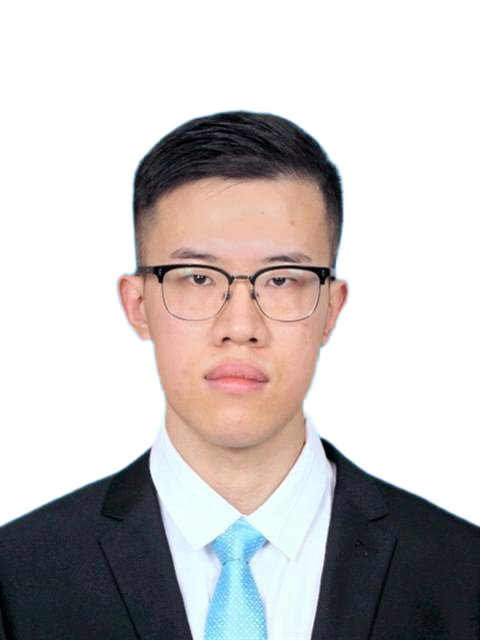
\includegraphics[width=0.95in]{resume_ch-master/picold.jpg}
\end{minipage}

% \section{\faGraduationCap\ 教育背景}
\section{\textbf{\stk{教育背景}}}
\begin{itemize}
  \item \datedsubsection{\textbf{\stk{北京大学|}}\stk{工程力学,理学博士}}{\stk{北京,中国|}2020.09 - \stk{至今}}\\
  \begin{itemize}[leftmargin=2.0pc]
    \item \stk{学术经历:主要从事颗粒物质、计算物理、离散元模拟研究;\textbf{\stk{耶鲁大学联合培养(2023.10 - 至今)}}}
    %\item \stk{荣誉奖励:北京大学校长奖学金、国家留学基金委奖学金、李惠荣奖学金、优秀科研奖(2次)}
    \item \stk{主要课程:机器学习、深度学习技术与应用、计算智能、并行程序设计、工程数据分析}
    %\item \stk{校园职位:校学生台湾研究会会长、校学生记者团主编、博士班级班长、院团委组织部副部长}
    
  \end{itemize}

  \item \datedsubsection{\textbf{\stk{密歇根大学|}}\stk{应用数据科学,理学硕士}}{\stk{安娜堡,美国|} \stk{2024秋入学}}\\
  % \begin{itemize}[leftmargin=2.0pc]
  %   \item \stk{主要课程:自然语言处理、强化学习、数据库架构与技术、云计算、大数据、数据挖掘}
  % \end{itemize}

  \item \datedsubsection{\textbf{\stk{佐治亚理工学院|}}\stk{计算科学-机器学习,理学硕士}}{\stk{亚特兰大,美国|}\stk{2024秋入学}}\\
  % \begin{itemize}[leftmargin=2.0pc]
  %   \item \stk{主要课程:计算机视觉、机器人与人工智能技术、贝叶斯方法}
  % \end{itemize}
    
  \item \datedsubsection{\textbf{\stk{北京大学|}}\stk{理论与应用力学,理学学士}}{\stk{北京,中国|}2016.09 - 2020.06}\\
  \begin{itemize}[leftmargin=2.0pc]
    \item \stk{主要课程:数学分析、程序设计、数据结构与算法、概率与数理统计}
  \end{itemize}

\end{itemize}

\section{\textbf{\stk{实习经历}}}
\begin{itemize}
  \item \datedsubsection{\textbf{\stk{KASUT PRADA Lab (可信智能与数据分析实验室),合作研究者}}}{2024.04 - \stk{至今}}\\

  \begin{itemize}[leftmargin=2.0pc]
    \item \stk{基于Hofstede文化维度,通过表征工程方法优化Llama-3-7b模型,显著提升其在跨文化场景中的应用效果,无需微调}
    \item \stk{针对不同国家(美国、中国、阿拉伯)训练Reward Model,并通过表征编辑微调大模型,显著改善大模型在跨文化数据上的表现}
  \end{itemize}
\end{itemize}

\section{\textbf{\stk{项目经验}}}
\begin{itemize}

\item \datedsubsection{\textbf{\stk{Kaggle - LMSYS - Chatbot Arena Human Preference Predictions (银牌)}}}{2024.07 - 2024.08}\\
\begin{itemize}[leftmargin=2.0pc]

    \item \stk{基于对话数据集预测人类偏好,采用QLoRA方法微调gemma2-9b与llama3.1-8b两个模型}
    \item \stk{调整超参数(学习率,模块冻结、prompt长度等)并保存最优训练权重,将两个模型加权融合}

\end{itemize}

\item \datedsubsection{\textbf{\stk{Kaggle - Image Matching Challenge 2024 - Hexathlon (银牌)}}}{2024.05 - 2024.06}\\
  %\datedsubsection{\stk{项目执行者}}{2022.05 - 2022.10}
  \begin{itemize}[leftmargin=2.0pc]

    \item \stk{针对多种不同3D场景的图像数据集进行检索,使用预训练模型efficientnet-b6&b7的ImageNet权重提取图像数据特征,基于余弦距离筛选,根据相似度排序每个场景数据集前n张图像集}
    \item \stk{用两个办法提取与匹配图像的特征关键点,一是分别使用kornia的角点特征检测器CornerGFTT及AdaLAM算法,二是分别使用SuperPoint及SuperGlue算法,最后存储匹配成功的点对}
    \item \stk{排除上述两种方法内相同点对后叠加,输入pycolmap计算最终的3d空间位置关系}
  \end{itemize}

% \item \datedsubsection{\textbf{\stk{基于强化学习的最密填充探索}}}{2022.05 - 2022.10}\\
%   %\datedsubsection{\stk{项目执行者}}{2022.05 - 2022.10}
%   \begin{itemize}[leftmargin=2.0pc]
%     \item \stk{对于椭球的最密晶胞填充,将传统贪心算法拓展到强化学习框架下,并耦合了无重叠安全约束}
%     \item \stk{对晶胞-颗粒系统进行Bi-level优化。结果未能达到贪心算法的精度,但填充密度接近}
%   \end{itemize}
  
  \item \datedsubsection{\textbf{\stk{局部有序结构的无监督学习算法}}}{2021.03 - 2022.01}\\
  %\datedsubsection{\stk{项目参与者}}{2021.03 - 2022.01}

  \begin{itemize}[leftmargin=2.0pc]
    \item \stk{将颗粒填充的局部结构转为点云格式,通过满足旋转、位移和交换不变性的深度自编码器降维}
    \item \stk{提出新的无监督学习算法,利用高斯混合模型或HDBSCAN进行结构聚类,再基于点云网络PointNet对填充中的结构进行识别并分类,公开数据集准确率可达96\%}
  \end{itemize}
\end{itemize}

% \begin{onehalfspacing}
% \end{onehalfspacing}

% \datedsubsection{\textbf{DID-ACTE} 荷兰莱顿}{2015年3月 - 2015年6月}
% \role{本科毕业设计}{LIACS 交换生}
% 利用结巴分词对中国古文进行分词与词性标注,用已有领域知识训练形成 classifier 并对结果进行调优
% \begin{onehalfspacing}
% \begin{itemize}
%   \item 利用结巴分词对中国古文进行分词与词性标注
%   \item 利用已有领域知识训练形成 classifier, 并用分词结果进行测试反馈
%   \item 尝试不同规则,对 classifier 进行调优
% \end{itemize}
% \end{onehalfspacing}

\section{\textbf{\stk{科研成果}}}
% increase linespacing [parsep=0.5ex]
\begin{itemize}[parsep=0.2ex]
  \item \textbf{Huang, Z.}, Deng, W., Zhang, S., \& Li, S. (2023). \textbf{Optimal shapes of disk assembly in saturated random packings}. \textit{Soft Matter}, 19(18), 3325-3336.
  \item Wang, Y., Deng, W., \textbf{Huang, Z.}, \& Li, S. (2022). \textbf{Descriptor-free unsupervised learning method for local structure identification in particle packings}. \textit{The Journal of Chemical Physics}, 156(15).
  \item \textbf{Huang, Z.}, Deng, W., Yuan, Y., Liu, L., Wang, Y., \& Li, S. (2022). \textbf{Determining the equivalent packing diameter of two-dimensional shapes}. \textit{Powder Technology}, 396, 565-577.
\end{itemize}


% \section{\faCogs\ IT 技能}
\section{\textbf{\stk{个人技能}}}
% increase linespacing [parsep=0.5ex]
\begin{itemize}[parsep=0.2ex]
  \item \textbf{\stk{编程语言}}: Python, C/C++, SQL%\stk{(熟悉数据结构与算法)}
  \item \textbf{\stk{工具与框架结构}}: TensorFlow, PyTorch, MATLAB, Git, Linux, PostgreSQL 
  \item \textbf{\stk{证书与语言}}: \stk{TensorFlow开发者专业证书、TensorFlow高级技术专项、\stk{托福} - 101/120}
\end{itemize}


% \end{itemize}

% \section{\faHeartO\ 项目/作品摘要}
% \section{项目/作品摘要}
% \datedline{\textit{An Integrated Version of Security Monitor Vis System}, https://hijiangtao.github.io/ss-vis-component/ }{}
% \datedline{\textit{Dark-Tech}, https://github.com/hijiangtao/dark-tech/ }{}
% \datedline{\textit{融合社交网络数据挖掘的电视节目可视化分析系统}, https://hijiangtao.github.io/variety-show-hot-spot-vis/}{}
% \datedline{\textit{LeetCodeOJ Solutions}, https://github.com/hijiangtao/LeetCodeOJ}{}
% \datedline{\textit{Info-Vis}, https://github.com/ISCAS-VIS/infovis-ucas}{}

\section{\textbf{\stk{更多信息}}}
\begin{itemize}[parsep=0.2ex]
  \item \textbf{\stk{荣誉奖励}}: \stk{北京大学校长奖学金、国家留学基金委奖学金、李惠荣奖学金、优秀科研奖(2次)}
  \item \textbf{\stk{学生工作}}: \stk{校学生台湾研究会会长、校学生记者团主编、博士班级班长、院团委组织部副部长} 
\end{itemize}

% \section{\textbf{\stk{个人总结}}}
% \stk{本人在校成绩优秀、性格开朗、踏实负责、勇于探索;具备出色沟通能力及组织能力,也具备较强的团队合作能力;数理基础和编程功底扎实,逻辑思维缜密,对人工智能及数据科学有极强的兴趣。}


%\section{\faInfo\ 社会实践/其他}
% \section{社区参与/实践其他}
% % increase linespacing [parsep=0.5ex]
% \begin{itemize}[parsep=0.2ex]
%   \item 乐于参与开源社区讨论,\textbf{参与翻译 Vue.js, webpack, WebAssembly, Babel 文档,印记中文成员}
%   \item 中国科学院大学2016秋季学期可视化与可视分析课程助教,\textit{http://vis.ios.ac.cn/infovis-ucas/}
%   \item 未来论坛学生会成员、北理社联新闻信息中心主任、北理工软件学院学生会宣传部副部长(2012-2016)
%   \item 2013-2015 北京市共青团“温暖衣冬”志愿者,第九届园博会志愿者,2014 FLL机器人世锦赛志愿者
% \end{itemize}

%% Reference
%\newpage
%\bibliographystyle{IEEETran}
%\bibliography{mycite}
\end{document}
